\section{eCAD GUI}
A graphical user interface (GUI) is a type of user interface that allows people to interact with a computer system by the use of graphical icons, visual indicators or special graphical elements called widgets, along with text and labels.The various actions are performed through direct manipulations of the graphical items like windows, buttons, menus, scroll bars, etc. GUI operations are much easier to use as user need not to know or memorize various commands. It contains a windows manager that allows user to display multiple-window areas. Each window runs a different process containing either a graphical or non-graphical display.\\

I created the GUI for GDCAD (now eCAD). In this project, first of all a rough sketch is made so that what is to made should be clear to the designer. The entire GUI is created in Qt, for that I go through the documentation of Qt which made me clear about how Qt is used for making GUI.\\\\

\begin{figure}[!ht]
\centering
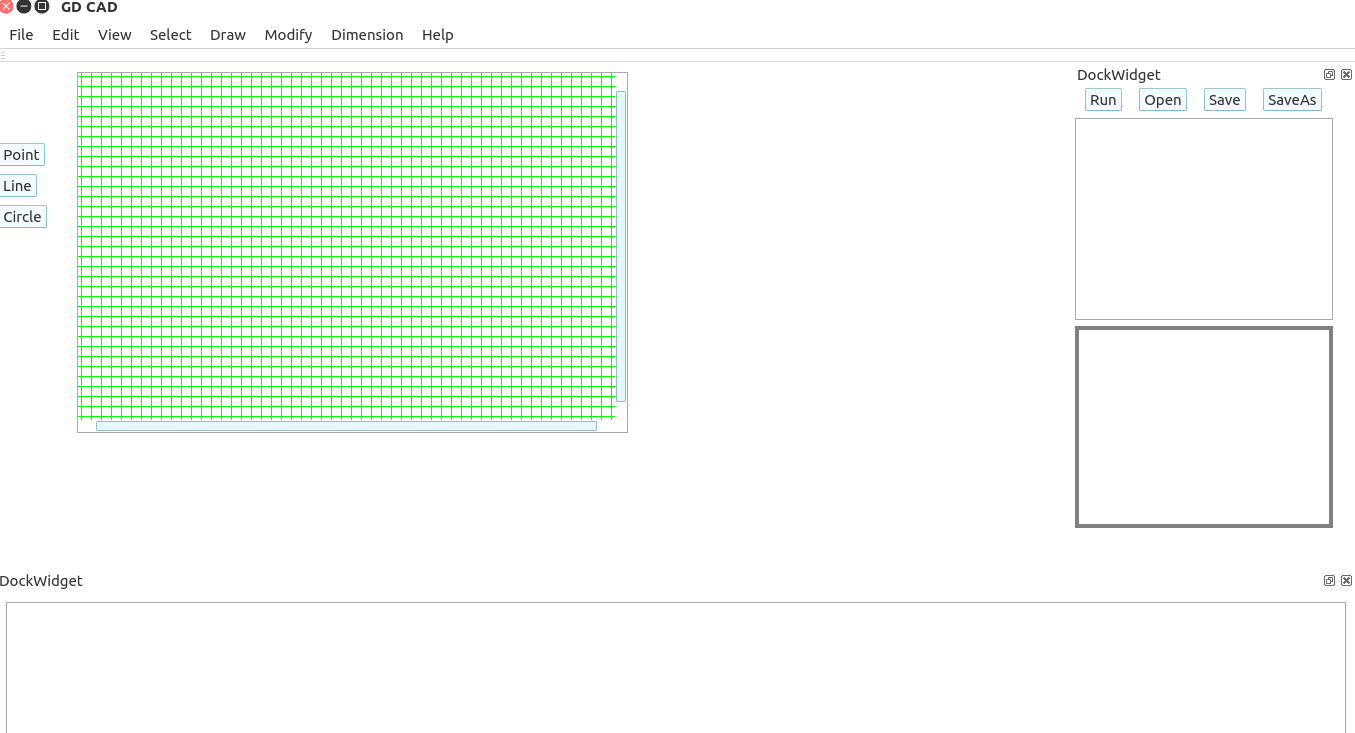
\includegraphics[width=0.9\textwidth]{images/gdcad.png}                   
\caption{GDCAD GUI (now changed)}
\end{figure}

The GDCAD GUI contains a main window which is further divided into different parts- Central Window, Script Dock Widget, Left toolbar containing different tools by clicking on them certain operations are performed, Command window from where user could enter a command like line, circle, etc and it would ask the user the required points according to the entity entered and last the status bar which contains the mouse pointer location. The entire GDCAD Gui was based on LibreCADv3, but due to certain change in plans or different approach according to our mentor the project name is changed to eCAD, which is entirely differnt from GDCAD in terms of GUI, so the new GUI is created for eCAD which consists of Tabbed document Interface (TDI) like the one in browers so that that at a time user can work on differnt windows. It contains various entities like point, circle, line, ellipse and text, remaining entities will also be included as the project is still under development stage and many features are included into it like undo, redo command, print and print preview option, load/save feature, etc.\\\\

\begin{figure}[!ht]
\centering
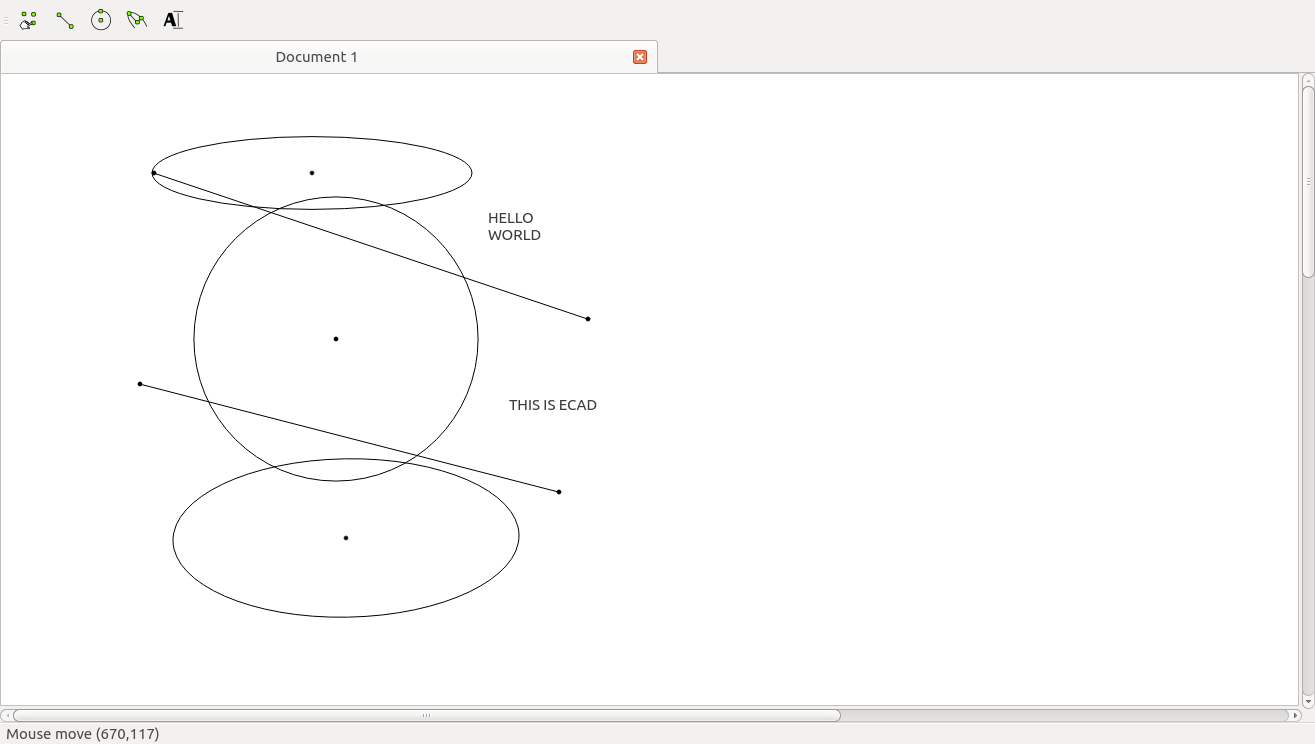
\includegraphics[width=0.9\textwidth]{images/ecad.png}                   
\caption{eCAD GUI (currently)}
\end{figure}
